\documentclass[12pt]{extarticle}
\usepackage{manualdoprofessor}
\usepackage{fichatecnica}
\usepackage{lipsum,media9,graficos}
\usepackage[justification=raggedright]{caption}
\usepackage[one]{bncc}
\usepackage[papagaio]{../edlab}
\usepackage{hyperref,graphicx}

\begin{comment}
Atividades
http://portaldoprofessor.mec.gov.br/storage/materiais/0000011867.pdf
https://www.bbc.com/portuguese/internacional-50842940

\end{comment}

\begin{document}


\newcommand{\AutorLivro}{Luis Marra}
\newcommand{\TituloLivro}{Crônicas do crack}
\newcommand{\Tema}{Diálogos com a sociologia e com a antropologia}
\newcommand{\Genero}{Conto, crônica e novela}
\newcommand{\imagemCapa}{./images/PNLD0027-01.png}
\newcommand{\issnppub}{---}
\newcommand{\issnepub}{---}
% \newcommand{\fichacatalografica}{PNLD0027-00.png}
\newcommand{\colaborador}{{Eduardo Modesto de Carvalho, Bruno Gradella e Vicente Castro}}


\title{\TituloLivro}
\author{\AutorLivro}
\def\authornotes{\colaborador}

\date{}
\maketitle

\baselineskip=1.2\baselineskip\par

\begin{abstract}\addcontentsline{toc}{section}{Carta ao professor}
Este Manual tem como objetivo fornecer subsídios para o trabalho com a
obra literária \emph{Crônicas do Crack}, de Luis Marra.

Luís Marra é um médico psiquiatra, escritor e literato brasileiro, nascido no ano
de 1950 e que, desde 2002, trabalha com dependentes químicos, sobretudo
aqueles que vivem nas regiões das diversas cracôlandias existentes na cidade
de São Paulo. Entre suas obras publicadas, estão os livros \emph{O Coletivo
Aleatório} (2001), \emph{O Diário Perdido do Jardim Maia} (2008) e, a principal delas,
\emph{Crônicas do Crack} (2017).

\emph{Crônicas do crack} reúne vinte relatos colhidos pelo autor no contato com dependentes. 
As histórias, que para alguns leitores podem ser assustadoras, são basicamente reais ou 
contêm muito pouca ficção, e foram construídas a partir de depoimentos colhidos em 
atendimentos médicos e conversas informais. A intenção é de 
observar o mundo do dependente químico, tanto em suas “viagens” como em suas relações 
sociais, considerando o ambiente pelo qual transita, os ``estados de loucura'', 
as relações com a sociedade e muitas vezes com o crime. Para preservar o anonimato
das personagens todos os nomes foram trocados. 

No capítulo do livro ``Antônio Santiago: o dito e o oculto'', o morador de rua Antônio 
Santiago se utiliza de uma boa retórica e esbanja criatividade em um diálogo com o 
doutor para conseguir uns trocados. Segundo o autor, há algo de literário 
na busca constante por algo indefinido, por uma ``viagem'', 
uma loucura extremada, principalmente no flerte com o perigo e com a morte.

``O canto da noia'', que abre o livro, foi escrito após uma visita feita a uma cracolândia 
da Zona Leste de São Paulo, durante a qual o médico acabou fazendo uma consulta coletiva a céu aberto. 
Já para escrever ``Sobrevivente de Troia", último capítulo, autor colheu relatos de 
atividades com grupos de teatro. Ao final de cada crônica, seguem, em itálico, 
depoimentos pessoais, observações, opiniões, dados complementares, e tudo isso de maneira 
a compor o que se poderia livremente considerar como os “bastidores” de cada um dos textos.

Esperamos que o livro ajude a combater o estereótipo 
construído sobre dependentes químicos, em particular, do crack. 



\end{abstract}

\tableofcontents


\section{Atividades 1}

%\BNCC{EM13LP26}

\subsection{Pré"-leitura}

%\BNCC{EM13LGG302}
%\BNCC{EM13LGG704}
%\BNCC{EM13LP10}
%\BNCC{EM13LP19}

\paragraph{Tema} ``Precisamos falar sobre isso.'' 

\paragraph{Conteúdo} Depoimentos de diversos usuários de crack em 
fase de tratamento, com o objetivo de apresentar a história de 
vida pessoais diante do dilema do crack e da marginalização que ele causa. 

\paragraph{Objetivo} O principal objetivo desta atividade 
é fazer com que o aluno vislumbre a realidade do usuário de 
crack para além dos estereótipos difundidos geralmente 
pela mídia. 

\paragraph{Justificativa} Os alunos precisam 
entender a situação complexa que leva uma pessoa a se tornar um usuário de drogas. 
Nessa primeira atividade, 
que antecede a leitura dos contos literários sobre usuários de crack, 
é necessário abordar o assunto a partir dos conceitos e
preconceitos já estabelecidos pelos próprios alunos. 
Veremos na metologia a seguir que os alunos serão 
convidados a assistir um breve documentário produzido pelo 
próprio autor e psiquiatra Luis Marra. O intuito é apresentar 
os usuários como pessoas comuns, capazes de explicar o significado da droga 
do ponto de vista especificamente delas. Consideramos essa 
atividade fundamental como pré-leitura da obra literária proposta.

\paragraph{Metodologia}
	\Image{Abertura do documentário ``Crônicas do crack'', de Luis Marra, disponível 
	no \href{https://www.youtube.com/watch?v=47NIEsOO6qA}{Youtube}}.{PNLD0027-11}
	
		Propomos exibir aos alunos o documentário
		intitulado <<Crônicas do crack>> feito pelo próprio
		autor do livro. O filme pode ser visto no seguinte link:
		\url{https://www.youtube.com/watch?v=47NIEsOO6qA}

		O filme tem cerca de 24 minutos e consiste em uma série de depoimentos
		de usuários de crack sobre
		a droga, o uso dela, como se envolveram com ela, 
		a violência que muitas vezes sofreram e a
		tentativa (para todos nesses casos bem sucedida) de recuperação.

		Sugerimos que o professor assista também a entrevista que o autor
		deu para a TV Estadão, disponível nesse link: 
		\href{https://www.facebook.com/209792265728043/videos/1772581939449060}{facebook.com/metropoleestadao}. E que leia se possível a entrevista dada à revista Cult, nesse 
		link: \href{https://rotacult.com.br/2017/08/dr-luis-marra-fala-sobre-o-livro-cronicas-do-crack/}{rotacult.com.br}. Em seguida:
	\begin{enumerate}
		\item Antes da exibição do vídeo, atenção. Alguns depoimentos podem ser muito fortes e portanto solicitamos 
		ao professor que assista previamente e avalie se seus alunos 
		estão preparados. E que converse com eles sobre isso antes da apresentação.
		\item Ainda antes da exibição, discuta com eles alguns tópicos de
		maneira informal. 

		\begin{itemize}
			\item \textit{Qual o significado da palavra droga?} Discuta com eles então o conceito da 
			palavra droga. Lembre-os que ``droga'' 
			em grego, \textit{phármakon}, significa tanto remédio quanto veneno, ou ainda 
			encantamento mágico, como a que os deuses fazem com os homens (\textit{Odisseia}; 
			cap.4; linha 220). 
			Lembre-os também que qualquer ``droga 
			medicinal'' pode ser um remédio mas também um veneno, conforme as dosagens. 

			\item \textit{Quais as drogas que conhecemos?} Peça para fazerem uma lista. Peça para 
			pensarem em drogas alternativas, supostamente inofensivas; as novas drogas; 
			as drogas que não se usam mais; as drogas usadas em outras culturas; as drogas usadas
			por um curto período de tempo durante a guerra. Comente com eles sobre o 
			uso de drogas pelos soldados durante a segunda guerra mundial a partir do 
			artigo ``High Hitler: como o uso de drogas mudou o desfecho da 2ª Guerra'', 
			publicado na revista Super Interessante, acessível por esse link: 
			\href{https://super.abril.com.br/historia/high-hitler-como-o-uso-de-drogas-mudou-o-desfecho-da-2a-guerra/}{super.abril.com.br/historia}.

			\item \textit{Toda droga é ilítica?} Elenque com eles as drogas lícitas e ilícitas. Lembre-os 
			por exemplo que o álcool é ilícito em países muçulmanos, por questões de religião. 
			Apresente uma lista de países que não aceitam álcool e quais os motivos e limites. 
			Eis uma breve lista de países e razões distintas para a proibição do álcool 
			nesse link: \href{https://www.terra.com.br/vida-e-estilo/turismo/internacional/jornal-lista-10-paises-onde-bebida-alcoolica-e-proibida,a1aebf5da7afe310VgnVCM5000009ccceb0aRCRD.html}{terra.com.br/vida-e-estilo}. 
			E lembre-os, ainda, que alguns países estão discutindo 
			qual os limites do uso de drogas como a maconha. Caso ache importante 
			aprofundar esse tópico, sugerimos essa matéria da BBC/Brasil sobre 
			as mudanças recentes no Uruguai. Link: 
			\href{https://www.bbc.com/portuguese/internacional-50842940}{bbc.com}.
		
			\item \textit{O que é um ``drogado'', um ``viciado''?} Esta é a principal 
			questão da nossa atividade, uma vez que assistirão a depoimentos de 
			usuários. Tente levantar todos os tipos de estereótipos 
			que os alunos conhecem. \textit{Quais nomes vocês conhecem para drogado?}
			``Noia'', ``noínha'', ``drogado'', ``doidão'', ``alucinado''...
			
			\item \textit{Todo drogado é marginal?} \textit{A droga leva ao crime?} Por fim, trate da
			questão da criminalidade como um estereótipo. 

		\end{itemize}

		\item Exiba o filme. Caso não tenha equipamento adequado, divida a sala em grupos de quadro
		e peça para assistirem em um celular. 
		
		\item Após o filme, retome com eles as perguntas iniciais. Abra a discussão. 
		
    \end{enumerate}

	\paragraph{Tempo estimado} 50 minutos. 


\Image{Luis Marra, autor de \textit{Crônicas do Crack}.}{PNLD0027-15.png}


\subsection{Leitura} 

%\BNCC{EM13LGG103}
%\BNCC{EM13LP02}
%\BNCC{EM13LP48}

\paragraph{Tema} <<A lágrima por trás do gorro ninja>>

\paragraph{Conteúdo} Discussão sobre os personagens envolvidos no conto. 

\paragraph{Objetivo} Discutir como foi escrito o conto a partir da comparação entre 
o texto do conto e os ``bastidores''. Lembramos que cada conto apresentado no 
livro é seguido também de uma seção em que o autor explica quais foram as 
circunstâncias reais em que conheceu os personagens, e também a sua opinião médica
sobre o caso. 

\paragraph{Justificativa} Tratar da compreensão da trama e da matéria do conto. 
Discutir os limites entre ficção e relato pessoal e as características do 
gênero. 

\paragraph{Metodologia}
 O conto ``A lágrima por trás do gorro ninja'' narra a história de um menino denominiado 
 somente pelas iniciais do seu nome -- W.R.\,-- que, 
 humilhado por uma situação de \textit{bulling} na escola, é encorajado por um tio
 a portar uma arma para ``dar um guenta'' naqueles que o ameaçavam. Imbuído de coragem, 
 o menino, então, é convidado pelo tio para fazer ``um serviço''. Sem saber o que vai 
 acontecer, mas tomado pela curiosidade, o menino acompanha o tio em uma emboscada, 
 invade a casa de um rival e se vê obrigado a executar a sangue frio uma pessoa. 
 Imediatamente após à cena, o menino, que portava um gorro preto para não ser 
 identificado, escuta uma criança correndo. ``Tio, não mata meu pai'', pede 
 a criança. W.R.\,então chora por trás do gorro, sem que seu tio perceba. 
 O crime já havia sido cometido. W.R, que morava então próximo 
 à cena do crime, passa a acompanhar a vida do filho da vítima. A paranoia de ser vingado
 e morto, e a culpa por ter tirado a vida de um pai, o desconcertam por absoluto. 
 W.R. recorre ao crack. 

 W.R.~então chega no consultório do médico, 
 ainda transtornado com a cena que cometera, e totalmente comprometido pelo 
 uso do crack. 

  Segundo Luis Marra, 
\begin{quote}
\textit{W.R.\,entendeu muito bem, ainda mais quando eu fiz menção à palavra"-chave
``caráter'', e disse que aquela lágrima atrás do gorro ninja era uma
prova oculta e íntima do caráter que ele tinha. Aquela lágrima era um
bem precioso que nunca ninguém dele tiraria.}
\end{quote}

O conto então narra o que se passou na vida de W.R.\,antes de ele se tornar 
um ``viciado''. Considerando isso, propomos a sequência didática:  

   \begin{enumerate}
   	\item Peça aos alunos para ler em casa o conto ``A lágrima por trás do gorro ninja''. 
   	\item No dia da aula, peça para alguém explicar a trama do conto. 

   	\item Cite a primeira frase do livro: <<\emph{transcrevo, ou então reescrevo, algumas semanas depois, o que teria sido, aproximadamente, a confissão de {W.R}.>>}. 

   	\item Coloque as questões: 
   	(a) \textit{este texto é uma descrição, uma narrativa ou um conto?}
   	(b) \textit{é tudo verdade o que está narrado}? Lembre-se que o autor diz  
   	``transcrevo ou então reescrevo''. 
   	(c) \textit{E a fala do personagem W.R.\,é verdade ou ficção?} Utilize para isso a 
   	seguinte passagem dos comentários do autor, ao final do conto:
   	``\emph{Acredito sinceramente que {W.R.}\,não deva ter mentido. Ele não tinha
	muito a perder. Além do mais, o que veio mesmo dele foi uma confissão
	num momento de intensa verdade em que o paciente adicto grave não oculta
	suas sombras profundas porque se sente momentaneamente livre, porque
	está rendido na tragédia pessoal para a interlocução acolhedora, e
	também porque mobiliza o fito sublime de expor sua luz irrompendo da
	escuridão.}''.
 
   	\item Discuta em que momento o crack entra na vida de W.R. 
	\item 
	Peça para escreverem em casa um texto argumentativo sobre o que foi 
	debatido, trazendo elementos da reflexão conjunta em sala de aula, mas também ideias próprias.
	Convide-os a comparar o caso de W.R. com alguma história real que conheçam. 
	E em seguida, peça para escreverem sobre ``um caso'' semelhante que conheçam.
	Tome o cuidado, no entanto, de pedir para que troquem todos os nomes, laços de
	parentesco ou até mesmo localidades. E explique que o importante no texto 
	é a trama, não o caso particular. Diga para eles que convém 
	ao leitor não ficar preocupado se é tudo verdade ou não. Basta a 
	verossimilhança da história, isto é, ``impressão da verdade que a ficção 
	consegue provocar no leitor.'' (\href{https://pt.wikipedia.org/wiki/Verossimilhan%C3%A7a#:~:text=Verossimilhan%C3%A7a%20%C3%A9%20a%20impress%C3%A3o%20da,que%20acontecem%20na%20realidade%20vivida.}{Wikipedia, ``Verossimilhança''})
   \end{enumerate}
\paragraph{Tempo estimado} Uma aula de 50 min. 


\subsection{Pós"-leitura}

%\BNCC{EM13LGG102}
%\BNCC{EM13LGG303}
%\BNCC{EM13LGG402}
%\BNCC{EM13LGG703}
%\BNCC{EM13LP13}
%\BNCC{EM13LP14}
%\BNCC{EM13LP28}
%\BNCC{EM13LP29}
%\BNCC{EM13LP52}

\paragraph{Tema} E quando acontece perto de mim? 
\paragraph{Conteúdo} A leitura e discussão sobre a redação dos 
	próprios alunos sobre um caso semelhante. 
\paragraph{Objetivo} Fazer com que os alunos discutam sua própria produção escrita 
	sobre assunto semelhante: o convívio com histórias de violência que 
	envolvem usuários de crack. O foco deve estar na vida da pessoa e não 
	nas ações que elas cometeram durante ou após o uso das drogas. 
	A redação não deve ter uma relação causal, \textit{o personagem fez $A$ 
	porque usou a droga $B$; ou passou a usar droga $B$ porque fez isso ou aquilo.}"
\paragraph{Justificativa} Aprofundar a discussão sobre a constituição dos personagens 
	do livro por meio da emulação\footnote{} e escrita criativa. A partir 
	da pergunta ``e você também conhece algum caso parecido?'' a intenção 
	é fazer com que os alunos descubram na literatura um recurso para 
	entender e expressar o seu próprio entorno.
\paragraph{Metodologia}
	Ao ler o livro, percebemos que o autor Luís Marra abordou a
	questão das drogas de um panorama distinto do que este tema é geralmente
	tratado. Comumente, o assunto dos entorpecentes e da dependência química
	são tratados de um ponto de vista médico, ou como um problema social.
	Raramente, busca"-se ouvir o indivíduo, isto é, sua perspectiva no
	cotidiano de dependente químico, suas experiências diárias, sua
	história, seus sonhos e objetivos. Nesse sentido, a obra de Luís Marra
	humaniza pessoas que, em geral, são tratadas apenas como estatística. 
	Considerando isso como uma estratégia para se abordar o tema 
	com os alunos, proponha o seguinte: 
\begin{enumerate}
	\item Retome a redação solicitada na aula anterior. 
	\item Peça para um aluno que conte a história que escreveu, sem ler. 
	Lembre-os que é preciso ficcionalizar um pouco para não expor a pessoa. 
	Troca-se um nome, uma cidade, uma parte do enredo. 
	E em seguida, peça para que outro aluno leia em voz alta o que 
	esse aluno narrou.
	\item Em seguida, discuta as circunstâncias do fato narrado, 
	tal qual faz o autor após cada conto. 
	\item Recolha os relatos dos demais alunos. 
	\item Em uma segunda aula, conte você mesmo em sala de aula 
	três relatos sem mencionar o nome dos alunos. 
	\item Abra para um debate sobre a exclusão e da desumanização 
	dessas pessoas, pontuando possibilidades para retomar uma vida 
	melhor para esses indivíduos em condições precárias.
\end{enumerate}
\paragraph{Tempo estimado} Duas aulas de 50 minutos. 

\section{Atividades 2}

\Image{O livro aborda a temática da dependência química a partir 
da perspectiva do indivíduo (Marco Gomes; CC-BY 2.0)}{PNLD0027-04.png}

%\BNCC{EM13CNT201}
%\BNCC{EM13CNT303}
%\BNCC{EM13CHS101}
%\BNCC{EM13CHS102}
%\BNCC{EM13CHS106}
%\BNCC{EM13CHS401}


\subsection{Pré"-leitura}
\SideImage{O crack inibe a recaptação da dopamina alterando o 
funcionamento dos neurônios (Autor Desconhecido; Domínio Público)}{PNLD0027-05.png}

\paragraph{Tema} Conversando com uma pessoa que um dia usou crack

\paragraph{Conteúdo} Preparar um série de entrevistas a serem feitas a um
	adicto ou ``ex-adicto''. 

\paragraph{Objetivo} O objetivo dessa atividade é colocar os alunos no lugar 
	do autor, e fazer com que eles perguntem e investiguem, de maneira construtiva, 
	a história pessoal de um usuário de crack. E que se preparem 
	para fazer perguntas contundentes e interdisciplinares. 

\paragraph{Justificativa} Colocar os alunos diante de uma experiência real, 
	e fazer com que eles façam perguntas segundo suas histórias e a experiência
	literária que tiveram anteriormente com a máteria. Envolver demais 
	professores em um evento maior, numa discussão ampla sobre o assunto. 

\paragraph{Metodologia}

\begin{enumerate}
	\item Monte um comitê de professores e alunos que se encarregue de 
	localizar e convidar formalmente um usuário ou ex-usuário de crack 
	para uma conversa na escola.
	\item Preparem uma série de perguntas que serão feitas durante 
	o evento. Separe as questões entre as fases ``antes'', ``durante'' 
	e ``depois'' do crack
	\item Em conversa com o professor de geografia, analise o que há de 
	política pública na sua cidade. Proponha ao professor que apresente 
	os programas atuais, tais como ``Crack, é possível vencer'', cujas
	apresentações estão disponíveis no site do Ministério da Justiça. Links:
	\href{https://www.justica.gov.br/news/conheca-o-programa-crack-e-possivel-vencer}%
	{Conheça o programa crack, é possível vencer} e 
	\href{https://www.justica.gov.br/programas-e-planos/crack#:~:text=O%20Crack%2C%20%C3%A9%20poss%C3%ADvel%20vencer,%3A%20preven%C3%A7%C3%A3o%2C%20cuidado%20e%20autoridade.}{Programas e planos}.
	O professor pode recorrer ainda ao vasto relatório elaborado pelo IPEA para 
	apresentar aos alunos os resultados do programa. O texto assinado 
	pelo sociólogo Márcio Júlio da Silva Mattos está disponível 
	neste link: \href{https://www.ipea.gov.br/ppp/index.php/PPP/article/view/683}{ipea.gov.br}.
\end{enumerate}


\paragraph{Tempo estimado} A definir segundo o envolvimento dos professores. Sugestão é que 
	este seja um trabalho coordenado do trimestre. 

\subsection{Leitura}

\paragraph{Tema} A entrevista.

\paragraph{Conteúdo} Alunos recebem na escola uma pessoa que é ou já foi usuário de crack.

\paragraph{Objetivo} Fazer  com que os alunos dialoguem, tal qual o autor do livro, 
	com uma pessoa que teve uma
	experiência com o crack com o objetivo de investigar a sua história pessoal 
	e as razões que levam uma pessoa a fazer tal escolha, e também as consequências. 

\paragraph{Justificativa} Se nas etapas anteriores, passamos do preconceito à experiência;
	da experiência à literatura; da literatura às narrativas pessoais dos alunos; agora
	nessa etapa, nosso objetivo é colocar os alunos na posição de entrevistadores
	e investigadores de um mundo pessoal afetado pela droga. Ao realizar uma entrevista, 
	os alunos serão obrigados a pesquisar sobre o que perguntar de maneira concisa e profunda, 
	tal qual puderam ver em entrevistas e também no livro. Eis as etapas da atividade:

\begin{enumerate}
	\paragraph{Metologia} 
	\item Escolham o nome, definam o dia e divulguem na escola o evento. 
	\item Convidem os alunos de uma faixa etária adequada. 
	\item Escolham um professor e um aluno para receber o convidado. 
	\item Criem uma equipe para registrar o evento, desde que o convidado
		aceite ser filmado. 
	\item Proponham ao convidado que fale da sua vida principalmente antes do crack e
		não foquem em questões técnicas e curiosidades banais sobre a droga. 
	\item Por fim, exponham as questões que foram discutidas anteriormente, 
		com os professores das áreas de humanidades. 
\end{enumerate}

\paragraph{Tempo estimado} Três horas.


\Image{Substâncias químicas e o corpo humano (Drug Disposal; Domínio Público)}{PNLD0027-06.png}


\subsection{Pós"-leitura}

\paragraph{Tema} Registro do evento

\paragraph{Conteúdo} Gravações dos evento, e transcrição e publicação da entrevista. 

\paragraph{Objetivo} Registrar a entrevista. 

\paragraph{Justificativa} Guardar e compartilhar o registro de uma experiência multidisciplinar 
	dos alunos. 

\paragraph{Metodologia}
	\begin{enumerate}
		\item Monte um grupo para a transcrição da entrevista. 
		\item Publique a entrevista com fotos no site medium.com
		\item Inclua num bloco de textos separado os ``bastidores'' da entrevista, ou seja, 
		as principais discussões antes e depois da entrevista. 
		\item Edite e publique a entrevista no Youtube, no canal da escola. 
		\item A publicação ou parte dela pode ser veiculadas no jornal da escola,
		serem expostas em um mural, ou mesmo no site do colégio.
	\end{enumerate}

\paragraph{Tempo estimado} Três aulas de 50 min., afora atividades em casa. 


\section{Aprofundamento}

% Ao chegar ao Ensino Médio, é necessário que os estudantes se aprofundem
% na compreensão das múltiplas linguagens e, sobretudo, da linguagem
% literária. Em relação à literatura, a \textsc{bncc} traz as seguintes
% considerações:

% \begin{quote}
% {[}\ldots{]} a leitura do texto literário, que ocupa o centro do trabalho
% no Ensino Fundamental, deve permanecer nuclear também no Ensino Médio.
% Por força de certa simplificação didática, as biografias de autores, as
% características de épocas, os resumos e outros gêneros artísticos
% substitutivos, como o cinema e as \textsc{hq}s, têm relegado o texto literário a
% um plano secundário do ensino. Assim, é importante não só (re)colocá"-lo
% como ponto de partida para o trabalho com a literatura, como
% intensificar seu convívio com os estudantes. Como linguagem
% artisticamente organizada, a literatura enriquece nossa percepção e
% nossa visão de mundo. Mediante arranjos especiais das palavras, ela cria
% um universo que nos permite aumentar nossa capacidade de ver e sentir.
% Nesse sentido, a literatura possibilita uma ampliação da nossa visão do
% mundo, ajuda"-nos não só a ver mais, mas a colocar em questão muito do
% que estamos vendo/vivenciando. (Brasil, 2018, p. 491)
% \end{quote}

Nesta seção, desenvolvemos um trabalho de aprofundamento que, em diálogo
com a formação continuada de professores, oferece subsídios para a
abordagem do texto literário. A leitura em sala de aula de
\emph{Crônicas do Crack} pode ser enriquecida pelo aprofundamento no
universo literário em que a obra está inserida.

\subsection{A obra}

O livro As crônicas do crack é uma composição de relatos colhidos
pelo médico psiquiatra Luis Marra, que trabalha com dependentes químicos
desde o ano de 2002. A forma de escrita destes relatos contidos dentro
do livro nos remete a algo bem literário, com uso de metáforas,
analogias e descrições. Ao olharmos para trechos do livro, vemos que ele
não é voltado para debater políticas públicas acerca do consumo de crack
na cidade de São Paulo, mas que o objetivo do autor é mirar no mundo do
dependente químico, nas suas ``viagens'', em suas relações sociais, no
ambiente em que ele está vivendo e até mesmo em sua própria loucura.

Dentro desta perspectiva, a escrita busca acabar com o estereótipo
construído de que a pessoa que consome crack é, única e exclusivamente,
um usuário. Assim, a obra denota que esses indivíduos têm sentimentos,
uma vida anterior ao vício, estando, muitas vezes, dentro de um contexto
desfavorável, além de indicar que o universo dos dependentes químicos
possui próprias relações de sociabilidade muito próprias.

\subsection{Um holofote a quem vive nas sombras}

Como já dito, o intuito e interesse do autor deste livro é mergulhar no
universo do dependente químico, sobretudo aquele que é usuário de crack.
Segundo suas próprias palavras em uma entrevista dada para a \textsc{tv} Estadão,
no ano de 2017: ``a pessoa viciada nesta droga contém dentro de si uma
criatividade tremenda''

\Image{Dependente químico mostrando cachimbo  (Marco Gomes; CC-BY 2.0)}{PNLD0027-08.png}

Isso fica claro ao leitor no capítulo do livro ``Antônio Santiago: o
dito e o oculto'', onde o morador de rua Antônio Santiago se utiliza de
uma boa retórica e esbanja criatividade em um diálogo com o doutor para
conseguir uns trocados. Além do mais, ainda segundo o médico, o
dependente se aproxima muito daqueles autores e pensadores que
vivenciaram o movimento literário do romantismo no século \textsc{xix}, por
sempre estar buscando a viagem, a loucura extremada e o flerte com o
perigo e com a morte.

\subsection{Uma questão social ampla e complexa}

Outro ponto que vale ser debatido é de que as drogas transitam por todas
as classes sociais. A ideia de que o consumo era exclusivo das classes
mais baixas já foi, há muito, posto de lado. Entretanto, não se
individualizou o dependente. Deve ser superada também a ideia de um
único perfil de dependente químico, existem vários perfis. Isso porque
as pessoas são individuais, apesar de elementos em comum, cada indivíduo
tem suas particularidades.

\Image{Moradores de rua no centro de São Paulo (Marco Gomes; CC-BY 2.0)}{PNLD0027-07.png}

Contudo, não se pode perder de vista que condições sociais podem
ocasionar maior ou menor peso para o consumo, vício, e superação deste.

Neste sentido, o norte"-americano Carl Hart, professor de psicologia pela
Universidade de Columbia e um dos especialistas no assunto nos diz que a
importância do ambiente em que o dependente químico está inserido é
crucial para o seu vício.

Dentro de um ambiente onde há diferentes alternativas que possam superar
o uso de drogas, a pessoa terá mais facilidade para sair da dependência.
Isto é evidenciado na obra em questão, já que o autor também nos mostra
as consequências dos ambientes e contextos com os quais os usuários
convivem.

Sendo assim, o autor ressalta que existe uma grande dificuldade com
relação a ajudar os dependentes químicos em condição de rua a superar a
dependência, posto que o ambiente em que estão inseridos é totalmente
desfavorável ao abandono dos psicoativos, sendo estimado que menos de
30\% dos usuários busquem tratamento ou qualquer tipo de ajuda.

\subsection{Uma discussão atual}

O livro é publicado em um momento em que o uso de psicoativos se tornou
endêmico em alguns locais, como por exemplo São Paulo, que abriga em seu
centro um dos maiores pontos de consumo de entorpecentes a céu aberto.

\Image{Dependentes químicos na região da Cracolândia (Luciana Marinho/Flickr; CC-BY 2.0)}{PNLD0027-09.png}

Ademais, dentro do mencionado contexto há de se lembrar também que os
últimos anos houve acalorados debates acerca de políticas públicas para
dependentes químicos, especialmente os que se encontram em situação de
rua.

Questões quanto a utilização do sistema público de saúde, a setores
urbanos que os dependentes ocupam e em que medida o problema
retroalimenta a violência são alguns pontos que podem ser levantados
acerca desta complexa questão.

Reflexões e provocações como essa se encontram ao longo das páginas da
obra de Luis Marra, uma vez que colhe relatos de regiões extremamente
marginalizadas, onde o poder do Estado não chega, e também traz
histórias do centro da cidade, escancarando a diferença de atuação do
Poder Público em cada um dos contextos

Ademais, vale frisar que, ao mesmo tempo que se pensa na questão dos
psicoativos como um problema social, que afeta a vida de milhões de
pessoas pelo mundo, existem estudos atuais que denotam que a boa
engenharia química de substâncias proscritas pode aprimorar a eficácia
de tratamentos medicinais, de sorte que o debate fomentado por essa obra
é, atual e riquíssimo e, sem dúvida, polêmico.

Portanto, Crônicas do crack, como já foi dito, não é um livro destinado
a defender esta o aquela política pública acerca da questão dos
dependentes químicos. Sua função, embora tangencie esses pontos é mais
humanitária. A obra está voltada para o descobrimento de seu universo,
dos atores que fazem parte deste ambiente, de suas sociabilidades e
pensamentos.

Ainda assim, não podemos tirar este escrito do contexto de ações mais
brutas em relação aos dependentes químicos que vivem nas ruas de São
Paulo, sendo impossível retirar a atuação do Estado do cotidiano desses
habitantes da capital paulistana.

\subsection{Atividades para o aprofundamento da pesquisa}

\subsubsection{A atualidade de <<Conto de Escola>>, de Machado de Assis}

Muitas vezes o discurso pedagógico e a escola são interpretados
pelos alunos como moralizantes ou ``distante da realidade''. Quando
se aborda um tema como as drogas, então, essa tendência é ainda mais evidente, 
uma vez que para o aluno do Ensino Médio, em vias de se tornar independente, 
as experiências próprias ou as narradas por colegas sobre ``qual é 
a real'' são confrontadas com explicações didáticas. A luz disso, sugerimos 
o trabalho com o texto de Machado de Assis, ``Conto de Escola''. O conto narra
a história de jovens com dificulades para acompanhar o desenvolvimento escolar
e propensos à evasão. Mais do que isso, estamos falando de uma história de 
1840, em que os jovens estão expostos tal como hoje. O conto foi lido 
pelo próprio autor de \textit{Crônicas do crack} e pode ser escutado \href{https://soundcloud.com/jorge-sallum/condo-de-escola-machado-de-assis-lido-por-luis-marra}{nesse link}.\medskip

\noindent\href{https://soundcloud.com/jorge-sallum/condo-de-escola-machado-de-assis-lido-por-luis-marra}{%
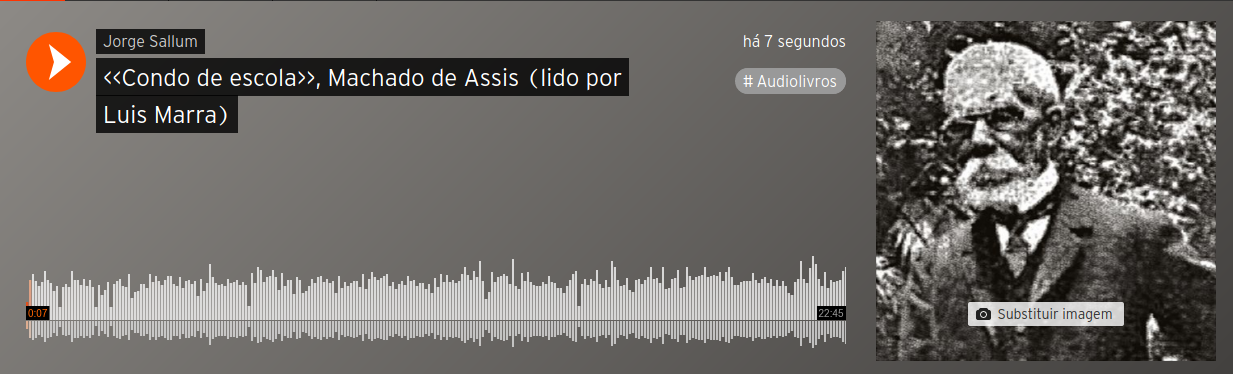
\includegraphics[width=\textwidth]{./images/PNLD0027-16}}

O texto de Machado de Assis pode ser lido no site:

\url{http://www.dominiopublico.gov.br/download/texto/ua000191.pdf}%
%{dominiopublico.gov.br}. 

Aconselhamos também que a professora ou professor leiam o capítulo 3,
``Machado de Assis e seu tempo'' e os subsequentes, do artigo do 
pesquisador Sidnei Ferreira de Vares, mestre em educação da FE-USP. 

\begin{quote}
O “Conto de Escola” constitui uma importante obra de nossa literatura, 
cujo fulcro temático é o sistema de ensino, mas especificamente a sala 
aula, onde se desenvolve a maior parte do conto. Nele, Machado expõe 
sua concepção de educação explorando as contradições existentes  
entre  a  realidade  da  escola  e  o  mundo  fora  dela.  Embora  o  
conto  não  traduza fielmente a trajetória do autor, pois não se 
trata de um texto biográfico, fornece informações até certo ponto 
precisas sobre a educação durante o período monárquico.

(\ldots{})

O  fio  condutor  do  conto  é  o  hiato  entre  a  natureza  infantil  
e  o  mundo  adulto,  cujos interesses  nem  sempre  coincidem.  
A  dúvida  que  paira  na  cabeça  infantil  de  Pilar  naquela 
manhã de maio de 1840, demonstra que suas preocupações imediatas não 
se aproximavam da escola. Brincar no campo de Sant'Anna ou no morro 
de São Diogo? Campo ou morro? Eis a questão  que  atormentava  o  menino  
e  que  em  nada  se  relacionava  com  os  estudos.
\end{quote}

Prepare então uma aula sobre Machado de Assis e a evasão escolar. 

\begin{itemize}	
	\item Apresente a situação da escola durante o Império (1822--1889). 
	Exemplifique com o caso específico do menino Machado de Assis, jovem 
	negro da cidade do Rio de Janeiro, com base no teto de Sidnei Ferreira. 
	\item Em seguida faça com que os alunos escutem o conto, lido pelo 
	escritor Luis Marra. Se possível, imprima partes do conto que lhe 
	interessar e distribua para os alunos. 
	\item Comente uma passagem específica do conto, como por exemplo as seguintes:

\begin{quote}
Raimundo  deu-me  a  pratinha,  sorrateiramente;  eu  meti-a  na  
algibeira  das calças, com um alvoroço que não posso definir. Cá 
estava ela comigo, pegadinha à perna. Restava prestar o serviço, 
ensinar a lição e não me demorei em fazê-lo, nem o  fiz  mal,  
ao  menos  conscientemente;  passava-lhe  a  explicação  em  
um  retalho  de papel que ele recebeu com cautela e cheio de 
atenção. Sentia-se que despendia um esforço  cinco  ou  seis  
vezes  maior  para  aprender  um  nada;  mas  contanto  que  
ele escapasse ao castigo, tudo iria bem.
\end{quote}

\begin{quote}
Rato  na  casaca...  Não  fui  à  escola,  acompanhei  os  
fuzileiros,  depois  enfiei pela Saúde, e acabei a manhã na Praia 
da Gamboa. Voltei para casa com as calças enxovalhadas,  sem  
pratinha  no  bolso  nem  ressentimento  na  alma.  E  contudo  
a pratinha  era  bonita  e  foram  eles,  Raimundo  e  Curvelo,  que  me  
deram  o  primeiro conhecimento, um da corrupção, outro 
da delação; mas o diabo do tambor..					
\end{quote}	
	
	\item Em seguida discuta com os alunos alguns paralelos entre
	os personagens narrados por Marra no conto 
	``Uma lágrima por trás do gorro ninja'' de Luis Marra e o 
	conto de Machado de Assis. 

\end{itemize}

\subsubsection{Debater a questão da internação sem autorização do paciente}

No dia 6 de junho de 2019, foi publicada a Lei 13.840/19, que permite
a internação compulsória de dependentes químicos, ou seja, sem a
necessidade de autorização judicial.

Desde sua concepção tal lei causou polêmica, uma vez que determinar a
internação compulsória gera impactos legais, sociais, morais e
econômicos. O princípio da legalidade encontra"-se expresso no texto
constitucional. De certo modo, a existência de uma lei supre a questão.
Entretanto, há um espectro nebuloso na discussão. Como se determinar
quando o indivíduo é dependente químico? Ademais, há a questão de até
que ponto o tratamento forçado realmente surte efeito, uma vez que o
dependente pode não ter interesse em se tratar. Por outro lado, é uma
forma de proteger as famílias que são expostas a comportamentos
perigosos do usuário. Assim, professor, nota"-se que é um assunto
polêmico. Outrossim, sua discussão é fundamental, posto que é tema da
contemporaneidade, devendo, portanto, ser debatido e aprofundado. Isso
posto, indica"-se a divisão da sala em grupos, cada qual, procurará
notícias e pareceres sobre o tema, segundo eixos temáticos, como por
exemplo, legal, médico, social, moral, econômico. Isso posto, todos
deverão expor aquilo que encontraram e, ao final, sugere"-se que a sala
seja colocada em roda, e que, a partir daí, se proponha uma discussão
sobre o tema, com o professor como mediador.

\Image{Entorno da Cracolândia (Marco Gomes; CC-BY 2.0)}{PNLD0027-10.png}

\subsubsection{Discussão sobre os riscos da droga}

A obra leva o leitor ao universo do dependente químico, oferecendo
assim grande subsídio para se entender seu mundo e sua rotina. Como
todo psicoativo, o crack atua junto ao sistema nervoso central,
ocasionando sensações de prazer, sendo uma das drogas com maior poder
de adição para o usuário. E como toda a droga, é imbuída de um ritual
social em sua utilização. Diante disso, é importante, até mesmo para
uma plena conscientização dos seus riscos, que o professor, juntamente
com os professores de ciências humanas e ciências da natureza, propor
uma roda de conversa com os alunos, onde se explicará o funcionamento
químico"-fisiológico dos entorpecentes no organismo, bem como os
aspectos sociais do consumo. Ao final, o aluno já plenamente
instrumentalizado, deverá redigir um texto, colocando sua opinião
sobre essa questão.

\section{Sugestões de referências complementares}\label{sugestoes}

\subsection{Livros}

\begin{itemize}
\item\textsc{bill}, M.V.; \textsc{soares}, Luiz Eduardo. \textit{Cabeça de Porco}. São Paulo: Objetiva, 2005.

O livro é o resultado de entrevistas e filmagens feitas ao longo de sete
anos em favelas brasileiras sobre crianças e jovens que vivem no mundo
do crime. Os relatos são associados aos textos do antropólogo Luiz
Eduardo Soares.

\item\textsc{loriga}, Ray. \textit{Héroes}. Alfaguara, 2014.

Um garoto se tranca em seu quarto para viver dentro da música, do que
lhe interessa, e fora de um mundo que lhe parece hostil.

\item\textsc{szabó}, Ilona; \textsc{clemente}, Isabel. \textit{Drogas: as histórias que não te contaram}. Rio de Janeiro: Zahar, 2017.

Através das trajetórias de cinco personagens conectadas pelo impacto da
cocaína, o livro traça um retrato complexo de um tema que ainda é tabu,
apresentando alternativas que vão além da repressão e do encarceramento.
\end{itemize}

\subsection{Filmes}

\begin{itemize}
\item\textbf{Aos treze}. Direção: Catherine Hardwicke (\textsc{eua}, 2013).

Inteligente e brilhante, Tracy se torna amiga da garota mais popular do
colégio, que a apresenta a um submundo de sexo, drogas e mutilação.
Nascerá uma nova Tracy, em conflito constante com colegas, professores
e, principalmente, com sua mãe.

\item\textbf{Bicho de sete cabeças}. Direção: Laís Bodanzky (Brasil, 2001).

Este premiado longa conta o drama de um relacionamento difícil entre pai
e filho, que leva este a ser mandado para um manicômio.

\item\textbf{Maria cheia de graça}. Direção: Joshua Marston (\textsc{eua}, Colômbia, 2004).

Grávida e desempregada, a jovem Maria aceita a proposta de um conhecido:
transportar heroína para Nova York em seu próprio estômago.
\end{itemize}

\subsection{Sites}

\begin{itemize}
\item\url{http://www.apadd.org/}.

Além de trazer informações institucionais e canais para quem deseja
ajudar a associação, o site fala sobre prevenção, tratamentos e
capacitação de profissionais para atuar no campo de dependência e
drogas.

\item\href{http://www.senado.leg.br/noticias/Jornal/emdiscussao/dependencia-quimica/iniciativas-do-governo-no-combate-as-drogas/historia-do-combate-as-drogas-no-brasil.aspx}{senado.leg.br}.

A página conta a história do combate repressivo a substâncias tóxicas no
Brasil, que teve início ainda nos primeiros anos do século \textsc{xvii}.

\item\url{www.justica.gov.br/sua-protecao/politicas-sobre-drogas}

O site fornece informações detalhadas sobre a \textsc{senad} (Secretaria Nacional
de Políticas sobre Drogas), a \textsc{pnad} (Política Nacional sobre Drogas) e o
\textsc{funad} (Fundo Nacional Antidrogas).
\end{itemize}

\section{Bibliografia comentada}

\begin{itemize}
\item\textsc{cardoso}, Fernando. \textit{Encarceramento e guerra às drogas}. Rio de
Janeiro: Gramma, 2019.

O livro é um compilado de pesquisas que refletem sobre como o Direito
Penal tem sido operado para manter o discurso e as práticas de
segregação de determinadas pessoas a partir do encarceramento em massa e
da guerra às drogas.

\item\textsc{cunha}, Wagner. \textit{Dependência química}. São Paulo: Ideia e Ação,
2008.

O psicólogo relata sua própria experiência com drogas para responder
perguntas comuns sobre o assunto e propor um tratamento que passa pelo
estabelecimento de metas e pela anuência do dependente.

\item\textsc{huxley}, Aldous. \textit{As portas da percepção}. São Paulo: Biblioteca
Azul, 2015.

O livro que influenciou gerações detalha o efeito das drogas, em especial da mescalina, substância extraida do cacto mexicano Peyote, sobre os
sentidos deste consagrado escritor.

\item\textsc{quincey}, Thomas de. \textit{Confissões de um comedor de ópio}. São Paulo: \textsc{l\&pm}, 2001.

O escritor inglês fala de sua experiência com o ópio, de como ela lhe
pareceu uma revelação de verdade divina. Trata"-se de um estudo pioneiro
da interferência do subconsciente nos sonhos.

\item\textsc{sanz}, Marta et.al. \textit{Drogadictos}. Madri: Demipage, 2017.

O livro compila os escritos de doze autores espanhóis e
latino"-americanos, que escrevem sobre drogas, seus efeitos e
consequências. Cada um fala sobre uma droga, como a mescalina, o ópio, o
crack, o álcool e o sexo.

\item\textsc{venâncio}, Renato Pinto; \textsc{carneiro}, Henrique (org.). \textit{Álcool e drogas na história do Brasil}. São Paulo: Alameda Editorial, 2005.

Este livro traça um panorama do significado que o álcool e outras drogas
tiveram na história do país, abordando uma gama de práticas sociais que
vão da cura ao crime, da alimentação ao amor, da medicina à religião, da
biopolítica à geopolítica.
\end{itemize}

\end{document}

